\chapter{Динамикалық бағдарламалау}

\index{динамикалық бағдарламалау}

\key{Динамикалық бағдарламалау} --
толық ізденістің дұрыстығы мен ашкөз алгоритмнің жылдамдығын
біріктіретін әдіс. Егер есеп бірнеше қабаттасқан ішесептерге 
бөлінсе және әрқайсысы тәуелсіз шешілетін болса, онда динамилалық
бағдарламалауды қолдануға болады.

Динамикалық бағдарламалауды екі кезде қолданады:

\begin{itemize}
\item
\key{Оңтайлы жауапты іздеу}.
Барынша аз немесе барынша үлкен
жауапты тапқымыз келгенде қолданамыз.
\item
\key{Шешімдердің санын есептеу}.
Мүмкін болатын шешімдердің жалпы санын 
есептегіміз келгенде қолданамыз.
\end{itemize}

Ең алдымен динамикалық бағдарламалау оңтайлы жауапты
қалай іздейтінін көреміз, кейін дәл сол идеяны
шешімдердің жалпы санын есептегенде қолданамыз.

Динамикалық бағдарламалауды түсіну -- әр спорттық
бағдарламалаушы үшін үлкен жетістік, айтулы қадам. Бірақ негізгі идеясы қарапайым болғанымен, динамикалық бағдарламалауды түрлі есептерде қолдану барысына келгенде қиындық  туындайды. 
Бұл тарауда динамикалық бағдарламалаудың бастамасы болатын 
классикалық есептер жинағын ұсынамыз.

\section{Тиын жайлы есеп}

Алдымен 6-тарауда талқыланған есептен
бастайық. Мысалы,
бізге тиындардың жиыны берілген, қосындысы 
$n$ болатын тиындарды таңдауымыз керек. 
Тиындардың мәндері: $\texttt{coins}=\{c_1,c_2,\ldots,c_k\}$. 
''Ең аз дегенде қанша тиын қажет болады?'' - деген сұраққа жауап іздейміз.

Осыған дейін біз бұл есепті әрдайым мүмкін болатын ең
үлкен тиынды алатын ашкөз алгоритм арқылы шығардық.
Алгоритм әңгіме қазақтың төл валютасы -- тиындары туралы болған жағдайда
жұмыс істейтіне көзіміз жетті. Бірақ, тұтастай алғанда,
ол міндетті түрде тиімді  жауап бере бермейді.

Енді бұл есепті барлық тиын жинағына тиімді
жауап беретін динамикалық бағдарламалау арқылы 
шешу жолын қарастырайық. Динамикалық бағдарламалауда
болуы мүмкін барлық қосындыларды қарап шығатын рекурсиялық
функция негізге алынады. Бірақ, оның тиімділігі \emph{мемоизацияның} қолданасында,
яғни біз әр ішесепті бір рет қана есептейміз.

\subsubsection{Рекурсия анықтамасы}

Динамикалық бағдарламалаудың идеясы -- 
есепті кіші ішесептерге бөлу, оларды шығару,
жауаптарын біріктіретін рекурсиялық формуланы анықтау.
Тиын жайлы есепті қарапайым рекурсияға ауыстырсақ, шарты төмендегідей болады:
''Қосындысы $x$ болатын қанша минималды тиын алуымыз қажет?'' - деген сұраққа жауап іздейміз. 

$\texttt{solve}(x)$ -- қосындысы $x$ - ке тең
минималды тиындар санын қайтаратын функция. 
Функцияның мәндері тиындардың мәндеріне тәуелді. 
Мысалы, тиындар $\texttt{coins} = \{1,3,4\}$ болса,
функцияның алғашқы мәндері төмендегідей болады:

\[
\begin{array}{lcl}
\texttt{solve}(0) & = & 0 \\
\texttt{solve}(1) & = & 1 \\
\texttt{solve}(2) & = & 2 \\
\texttt{solve}(3) & = & 1 \\
\texttt{solve}(4) & = & 1 \\
\texttt{solve}(5) & = & 2 \\
\texttt{solve}(6) & = & 2 \\
\texttt{solve}(7) & = & 2 \\
\texttt{solve}(8) & = & 2 \\
\texttt{solve}(9) & = & 3 \\
\texttt{solve}(10) & = & 3 \\
\end{array}
\]

Үлгіде, $\texttt{solve}(10)=3$,
себебі қосындысы 10 болатындай 
ең кемінде 3 тиын қажет.
Оңтайлы жауап -- $3+3+4=10$.

$\texttt{solve}$ функциясының негізгі қасиеті --
функцияның мәндерін
кіші аргументтердің функциядағы мәндерінен есептеуі.
Идеясы -- қосынды үшін таңдайтын \emph{бірінші} тиынға назар аудару.
Мысалы, жоғарыдағы жағдайда бірінші тиын 1, 3 немесе 4
бола алады. Егер біз бірінші тиынды 1 деп алатын болсақ,
бізге қосындысы 9 болатын минималды тиындар санын білу қажет.
Ал ол -- негізгі есептің ішесебі. Демек минималды тиындар
санын санайтын төмендегідей рекурсиялық функция құрауымызға болады:
\begin{equation*}
\begin{split}
\texttt{solve}(x) = \min( & \texttt{solve}(x-1)+1, \\
                           & \texttt{solve}(x-3)+1, \\
                           & \texttt{solve}(x-4)+1).
\end{split}
\end{equation*}
Рекурсияның негізі $\texttt{solve}(0)=0$,
себебі нөл қосындысын құрау үшін тиын қажет емес. 
Мысалы,
\[ \texttt{solve}(10) = \texttt{solve}(7)+1 = \texttt{solve}(4)+2 = \texttt{solve}(0)+3 = 3.\]

Енді қосындысы $x$ болатын минималды тиындардың санын есептейтін
жалпы рекурсиялық функцияны анықтауға болады:
\begin{equation*}
    \texttt{solve}(x) = \begin{cases}
               \infty               & x < 0\\
               0               & x = 0\\
               \min_{c \in \texttt{coins}} \texttt{solve}(x-c)+1 & x > 0 \\
           \end{cases}
\end{equation*}

Біріншіден, егер $x<0$ болса, онда мәні $\infty$,
өйткені теріс сан қосындысын құрау мүмкін емес.
Келесі, егер $x=0$ болса мәні $0$ - ге тең,
себебі нөл қосындысын құрау үшін тиын қажет емес.
Соңында егер $x>0$ болса, $c$ айнымалысы 
қосындының бірінші тиын таңдауындағы барлық 
мүмкіндіктерінен өтіп шығады.

Есепті шығаратын рекурсиялық функция табылғаннан кейін
кодты С++ тілінде жазуымызға болады (\texttt{INF} тұрақтысы шексіздікті
білдіреді):

\begin{lstlisting}
int solve(int x) {
    if (x < 0) return INF;
    if (x == 0) return 0;
    int best = INF;
    for (auto c : coins) {
        best = min(best, solve(x-c)+1);
    }
    return best;
}
\end{lstlisting}

Дегенмен бұл функция тиімсіз, өйткені қосындыны құру тәсілдерінің экспоненциалды саны бар болуы мүмкін. Мемоизация арқылы функцияны оңтайлырақ
ете аламыз.

\subsubsection{Мемоизацияның қолданысы}

\index{мемоизация}

Динамикалық бағдарламалаудың идеясы --
\key{мемоизация} арқылы рекурсивтік функцияның
мәндерін жылдам есептеу, 
яғни функцияның әр параметрінің
мәнін бір рет есептеп, оның мәні қажет 
болған жағдайда жиымнан алу.

Есепте келесі жиымдарды қолданайық:
\begin{lstlisting}
bool ready[N];
int value[N];
\end{lstlisting}

Мұндағы $\texttt{ready}[x]$  $\texttt{solve}(x)$ мәні саналғанын немесе саналмағанын көрсетсе,
оның саналған жағдайдағы мәні $\texttt{value}[x]$ - те сақталады.
$N$ тұрақтысы барлық мәндерді қамтитындай етіп алынған.

Енді осы функцияны төмендегідей етіп, тиімдірек
жазуға болады:

\begin{lstlisting}
int solve(int x) {
    if (x < 0) return INF;
    if (x == 0) return 0;
    if (ready[x]) return value[x];
    int best = INF;
    for (auto c : coins) {
        best = min(best, solve(x-c)+1);
    }
    value[x] = best;
    ready[x] = true;
    return best;
}
\end{lstlisting}

Функцияның $x<0$ және $x=0$ негізгі жағдайларын 
бұрынғыдай өңдейміз. Содан соң функция
$\texttt{ready}[x]$ арқылы 
$\texttt{solve}(x)$ бұрын есептелгенін не есептелмегенін тексереді.
Егер есептелген болса, бірден $\texttt{value}[x]$
мәнін қайтаруға болады. Басқаша жағдайда функция рекурсия арқылы
$\texttt{solve}(x)$ мәнін есептеп, оның мәнін 
$\texttt{value}[x]$-ке сақтайды. 

Әр $x$ параметрі бір рет рекурсивті есептелгендіктен,
функция тиімдірек жұмыс жасайды. $\texttt{solve}(x)$ мәні 
$\texttt{value}[x]$-те сақталғаннан кейін
$x$ параметрімен функция тағы шақырылғанда, 
оны тиімді түрде алуға болады. уақытша күрделілігі
-- $O(nk)$, мұндағы $n$ қалаған қосыныдының мәні 
және $k$ тиындардың саны. 

\texttt{value} жиымын 
цикл арқылы \emph{итеративті} түрде
құрастыруға болатынын ескеріңіз:

\begin{lstlisting}
value[0] = 0;
for (int x = 1; x <= n; x++) {
    value[x] = INF;
    for (auto c : coins) {
        if (x-c >= 0) {
            value[x] = min(value[x], value[x-c]+1);
        }
    }
}
\end{lstlisting}

Спорттық бағдарламалаушылардың көп бөлігі өлшемі ықшам болып келетініне және тұрақты фактордың аздығына байланысты 
осы нұсқаны қолданғанды жөн көреді. 
Біз алдағы мысалдарда итеративті түрді де 
пайдаланатын боламыз.
Дегенмен динамикалық бағдарламалаудың шешімдерін 
рекурсивті ойлау әдетте жеңіл екенін есте сақтағанымыз дұрыс.

\subsubsection{Шешім құрастыру}

Кейде бізден есептің оңтайлы жауабы мен 
оған жететін үлгіні табуды сұрайды. 
Мысалы, тиын жайлы есепте бірінші тиын
қандай болатынын сақтайтын жаңа жиым ашуға
болады:
\begin{lstlisting}
int first[N];
\end{lstlisting}
Кейін алгоритмді төмендегідей өзгерте аламыз:
\begin{lstlisting}
value[0] = 0;
for (int x = 1; x <= n; x++) {
    value[x] = INF;
    for (auto c : coins) {
        if (x-c >= 0 && value[x-c]+1 < value[x]) {
            value[x] = value[x-c]+1;
            first[x] = c;
        }
    }
}
\end{lstlisting}

Төмендегі код қосындысы $n$ болатын
оңтайлы тиындарды көрсетеді:
\begin{lstlisting}
while (n > 0) {
    cout << first[n] << "\n";
    n -= first[n];
}
\end{lstlisting}

\subsubsection{Шешімдердің жолын санау}

Тиын жайлы есептің басқа түрін қарастырып 
көрейік. Бұл жерде ''тиындарды қолданып $x$ қосындысын
қанша жолмен алуға болады?'' - деген сұраққа жауап іздейміз. 
Мысалы тиындар $\texttt{coins}=\{1,3,4\}$ және
$x=5$ болса, 6 жол бар:

\begin{multicols}{2}
\begin{itemize}
\item $1+1+1+1+1$
\item $1+1+3$
\item $1+3+1$
\item $3+1+1$
\item $1+4$
\item $4+1$
\end{itemize}
\end{multicols}

Есепті қайтадан рекурсия арқылы шығаруға да болады.
$\texttt{solve}(x)$ функциясын $x$ қосындысын 
құруға болатын жолдардың саны деп белгілейік. 
Мысалы, тиындар $\texttt{coins}=\{1,3,4\}$,  $\texttt{solve}(5)=6$ және
рекурсивтік формула төмендегідей болса:
\begin{equation*}
\begin{split}
\texttt{solve}(x) = & \texttt{solve}(x-1) + \\
                    & \texttt{solve}(x-3) + \\
                    & \texttt{solve}(x-4)  .
\end{split}
\end{equation*}

Жалпы рекурсивтік функция келесі үлгідегідей болады:
\begin{equation*}
    \texttt{solve}(x) = \begin{cases}
               0               & x < 0\\
               1               & x = 0\\
               \sum_{c \in \texttt{coins}} \texttt{solve}(x-c) & x > 0 \\
           \end{cases}
\end{equation*}

Егер $x<0$ болса, онда мәні 0, себебі жауап жоқ.
Егер $x=0$ болса, онда мәні 1, себебі қосындысы 0 
болатын тек бір ғана жол бар.
Әйтпесе біз $\texttt{solve}(x-c)$ өрнегіндегі
барлық мәндер қосындысын есептеп шығамыз, 
мұндағы $c$ \texttt{coins} жиымының элементі. 

Төмендегі код параметрі $0 \le x \le n$ болатын
$\texttt{count}$ мәндерінен
құралған $\texttt{count}[x]$ жиымын құрастырады:

\begin{lstlisting}
count[0] = 1;
for (int x = 1; x <= n; x++) {
    for (auto c : coins) {
        if (x-c >= 0) {
            count[x] += count[x-c];
        }
    }
}
\end{lstlisting}

Әдетте жолдардың саны тым үлкен болғандықтан, 
оның нақты санын табу міндетті емес. Кей
есепте оның $m$-ға бөлінгендегі қалдығын сұрайды 
(мысалы $m=10^9+7$). Барлық есептеулер $m$ модулі бойынша 
орындалатындай етіп кодты өзгерте аламыз.

Жоғарыдағы кодта төмендегі жолдан кейін
\begin{lstlisting}
        count[x] += count[x-c];
\end{lstlisting}
келесі жолды жазсақ жеткілікті
\begin{lstlisting}
        count[x] %= m;
\end{lstlisting}

Біз динамикалық бағдарламалаудың 
барлық негізгі тақырыптарын талдадық.
Қолданыс аясы кең болғандықтан оның мүмкіндіктерін
көрсететін бірнеше есепті қарастырамыз.

\section{Ең ұзын өспелі іштізбек}

\index{ең ұзын өспелі іштізбек}

Бірінші есебіміз -- өлшемі $n$ болатын
жиымнан
\key{ең ұзын өспелі іштізбекті табу}.
Бұл -- ұзындығы максималды болатын жиым 
элементтері солдан оңға қарай өсу ретімен 
орналасқан тізбек.

Мысалы, төмендегі жиым 

\begin{center}
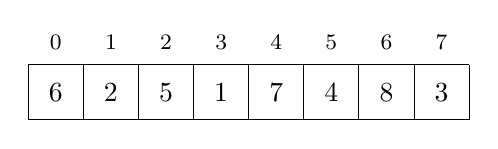
\begin{tikzpicture}[scale=0.7]
\draw (0,0) grid (8,1);
\node at (0.5,0.5) {$6$};
\node at (1.5,0.5) {$2$};
\node at (2.5,0.5) {$5$};
\node at (3.5,0.5) {$1$};
\node at (4.5,0.5) {$7$};
\node at (5.5,0.5) {$4$};
\node at (6.5,0.5) {$8$};
\node at (7.5,0.5) {$3$};

\footnotesize
\node at (0.5,1.4) {$0$};
\node at (1.5,1.4) {$1$};
\node at (2.5,1.4) {$2$};
\node at (3.5,1.4) {$3$};
\node at (4.5,1.4) {$4$};
\node at (5.5,1.4) {$5$};
\node at (6.5,1.4) {$6$};
\node at (7.5,1.4) {$7$};
\end{tikzpicture}
\end{center}
ең ұзын өспелі іштізбектің өлшемі 4 болады:
\begin{center}
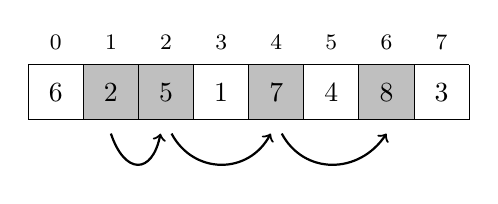
\begin{tikzpicture}[scale=0.7]
\fill[color=lightgray] (1,0) rectangle (2,1);
\fill[color=lightgray] (2,0) rectangle (3,1);
\fill[color=lightgray] (4,0) rectangle (5,1);
\fill[color=lightgray] (6,0) rectangle (7,1);
\draw (0,0) grid (8,1);
\node at (0.5,0.5) {$6$};
\node at (1.5,0.5) {$2$};
\node at (2.5,0.5) {$5$};
\node at (3.5,0.5) {$1$};
\node at (4.5,0.5) {$7$};
\node at (5.5,0.5) {$4$};
\node at (6.5,0.5) {$8$};
\node at (7.5,0.5) {$3$};

\draw[thick,->] (1.5,-0.25) .. controls (1.75,-1.00) and (2.25,-1.00) .. (2.4,-0.25);
\draw[thick,->] (2.6,-0.25) .. controls (3.0,-1.00) and (4.0,-1.00) .. (4.4,-0.25);
\draw[thick,->] (4.6,-0.25) .. controls (5.0,-1.00) and (6.0,-1.00) .. (6.5,-0.25);

\footnotesize
\node at (0.5,1.4) {$0$};
\node at (1.5,1.4) {$1$};
\node at (2.5,1.4) {$2$};
\node at (3.5,1.4) {$3$};
\node at (4.5,1.4) {$4$};
\node at (5.5,1.4) {$5$};
\node at (6.5,1.4) {$6$};
\node at (7.5,1.4) {$7$};
\end{tikzpicture}
\end{center}

$k$ позициясына бітетін
ең ұзын өспелі іштізбектің өлшемін $\texttt{length}(k)$ деп белгілейік.
Осылайша $\texttt{length}(k)$ функциясының 
$0 \le k \le n-1$ параметрлерінің мәндерін есептесек, 
жиымның ең ұзын өспелі іштізбегінің өлшемін
таба аламыз. Мысалы, 
жоғарыда келтірілген жиымдағы функцияның мәндері мынадай болады:

\[
\begin{array}{lcl}
\texttt{length}(0) & = & 1 \\
\texttt{length}(1) & = & 1 \\
\texttt{length}(2) & = & 2 \\
\texttt{length}(3) & = & 1 \\
\texttt{length}(4) & = & 3 \\
\texttt{length}(5) & = & 2 \\
\texttt{length}(6) & = & 4 \\
\texttt{length}(7) & = & 2 \\
\end{array}
\]

Мысалы, $\texttt{length}(6)=4$, себебі
6-позицияда бітетін ең ұзын өспелі іштізбек
4 элементтен тұрады.

$\texttt{length}(k)$ мәнін есептеу үшін
$i<k$ позциясында $\texttt{array}[i]<\texttt{array}[k]$
шарты орындалуы және $\texttt{length}(i)$ мүмкіндігінше
үлкен болуы қажет.
Бұдан
$\texttt{length}(k)=\texttt{length}(i)+1$ болатынын байқаймыз.
Бұл -- ішжиымға $\texttt{array}[k]$ - ні
қосудың тиімді жолы.
Бірақ $i$ табылмаса, $\texttt{length}(k)=1$ болады,
яғни іштізбектік тек $\texttt{array}[k]$ элементінен тұрады. 

Функцияның әр мәні оның кіші мәндерінен есептелетіндіктен
динамикалық бағдарламалауды қолдана аламыз. 
Төменде келтірілетін кодта функцияның мәндері $\texttt{length}$ 
жиымында сақталады.

\begin{lstlisting}
for (int k = 0; k < n; k++) {
    length[k] = 1;
    for (int i = 0; i < k; i++) {
        if (array[i] < array[k]) {
            length[k] = max(length[k],length[i]+1);
        }
    }
}
\end{lstlisting}

Кодтың уақытша күрделілігі -- $O(n^2)$, өйткені ол
екі кірістірілген циклден тұрады. 
Алайда дәл солай $O(n \log n)$ уақытта динамикалық бағдарламалаудың мәндерін анағұрлым тиімдірек 
есептеуімізге болады.
Ал сіз қандай жолдарын білесіз?

\section{Тордағы жолдар}

Біздің келесі есебіміз 
$n \times n$ торының жоғарғы сол жақ бұрышынан
төменгі оң жақ бұрышына дейін тек оңға және төменге
қозғалу арқылы жол табуға арналады. Әр 
шаршыда бір сан жазылған,
құрастырылған жолдағы сандардың
қосындысы максималды болуы қажет. 

Келесі сурет
тордағы оңтайлы жолды көрсетеді:
\begin{center}
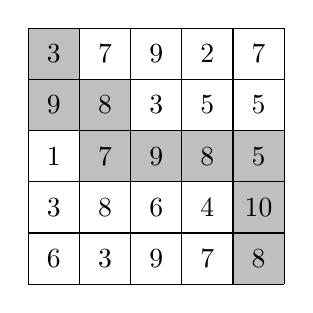
\begin{tikzpicture}[scale=.65]
  \begin{scope}
    \fill [color=lightgray] (0, 9) rectangle (1, 8);
    \fill [color=lightgray] (0, 8) rectangle (1, 7);
    \fill [color=lightgray] (1, 8) rectangle (2, 7);
    \fill [color=lightgray] (1, 7) rectangle (2, 6);
    \fill [color=lightgray] (2, 7) rectangle (3, 6);
    \fill [color=lightgray] (3, 7) rectangle (4, 6);
    \fill [color=lightgray] (4, 7) rectangle (5, 6);
    \fill [color=lightgray] (4, 6) rectangle (5, 5);
    \fill [color=lightgray] (4, 5) rectangle (5, 4);
    \draw (0, 4) grid (5, 9);
    \node at (0.5,8.5) {3};
    \node at (1.5,8.5) {7};
    \node at (2.5,8.5) {9};
    \node at (3.5,8.5) {2};
    \node at (4.5,8.5) {7};
    \node at (0.5,7.5) {9};
    \node at (1.5,7.5) {8};
    \node at (2.5,7.5) {3};
    \node at (3.5,7.5) {5};
    \node at (4.5,7.5) {5};
    \node at (0.5,6.5) {1};
    \node at (1.5,6.5) {7};
    \node at (2.5,6.5) {9};
    \node at (3.5,6.5) {8};
    \node at (4.5,6.5) {5};
    \node at (0.5,5.5) {3};
    \node at (1.5,5.5) {8};
    \node at (2.5,5.5) {6};
    \node at (3.5,5.5) {4};
    \node at (4.5,5.5) {10};
    \node at (0.5,4.5) {6};
    \node at (1.5,4.5) {3};
    \node at (2.5,4.5) {9};
    \node at (3.5,4.5) {7};
    \node at (4.5,4.5) {8};
  \end{scope}
\end{tikzpicture}
\end{center}
Жолдағы сандардың қосындысы 67-ге тең және 
бұл жол жоғарғы сол жақ бұрыштан
төменгі оң жақ бұрышқа апаратын ең үлкен қосынды бола алады.

Тордың жолдары мен бағаналары 1-ден $n$-ге дейін
белгіленген, $\texttt{value}[y][x]$ - тің мәні
$(y,x)$ шаршысында жазылған сан.
$\texttt{sum}(y,x)$ мәнін жоғарғы сол жақ бұрыштан
$(y,x)$ шаршысына дейінгі жолдағы 
максималды қосынды деп есептейік.
Сәйкесінше, $\texttt{sum}(n,n)$ мәні жоғарғы сол жақ 
бұрыштан төменгі оң жақ бұрышқа дейінгі 
максималды қосындыны көрсетеді.
Жоғарыда көрсетілген торда $\texttt{sum}(5,5)=67$.  

Қосындыларды рекурсивті түрде былайша санай аламыз:
\[ \texttt{sum}(y,x) = \max(\texttt{sum}(y,x-1),\texttt{sum}(y-1,x))+\texttt{value}[y][x]\]

Рекурсивті формула $(y,x)$ шаршысында 
аяқталатын жол $(y,x-1)$ шаршысынан немесе 
$(y-1,x)$ шаршысынан келетінін байқауға негізделген:

\begin{center}
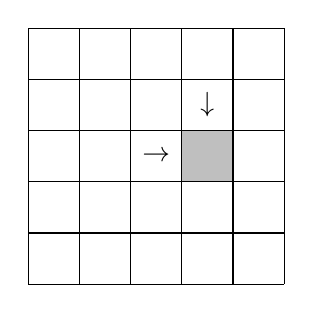
\begin{tikzpicture}[scale=.65]
  \begin{scope}
    \fill [color=lightgray] (3, 7) rectangle (4, 6);
    \draw (0, 4) grid (5, 9);
    
    \node at (2.5,6.5) {$\rightarrow$};
    \node at (3.5,7.5) {$\downarrow$};
    
  \end{scope}
\end{tikzpicture}
\end{center}

Демек біз қосындыны арттыратын бағытты таңдаймыз. 
Егер $y=0$ немесе $x=0$ болса, 
$\texttt{sum}(y,x)=0$ (себебі мұндай жол жоқ).
Сондықтан формула $y=1$ немесе $x=1$ болған кезде жұмыс 
жасай береді. 

\texttt{sum} функциясында екі параметр болғандықтан
динамикалық бағдарламалау жиымы екі өлшемдік болады.
Мысалы, төмендегі жиынды пайдалана отырып
\begin{lstlisting}
int sum[N][N];
\end{lstlisting}
қосындыны келесі үлгідегідей етіп есептей аламыз:
\begin{lstlisting}
for (int y = 1; y <= n; y++) {
    for (int x = 1; x <= n; x++) {
        sum[y][x] = max(sum[y][x-1],sum[y-1][x])+value[y][x];
    }
}
\end{lstlisting}
Мұндағы алгоритмнің уақытша күрделілігі -- $O(n^2)$.

\section{Қоржын жайлы есептер}

\index{қоржын}

\key{Қоржын} туралы есептерге объектілер жиыны 
берілген және белгілі бір қасиеттері бар 
ішжиындарды табу талап етілетін есептер жатады.
Әдетте оларды динамикалық бағдарламалау арқылы шығаруға болады.

Бұл бөлімде біз келесі есепті қарастырамыз:
$[w_1,w_2,\ldots,w_n]$ салмақтар тізімі берілген.
Салмақтарды пайдаланып құруға 
болатын барлық қосындыларды анықтау қажет. 
Мысалы, салмақтар жиымы $[1,3,3,5]$ болса,
төмендігей қосындыларды құрастыруға болады:

\begin{center}
\begin{tabular}{rrrrrrrrrrrrr}
 0 & 1 & 2 & 3 & 4 & 5 & 6 & 7 & 8 & 9 & 10 & 11 & 12 \\
\hline
 X & X & & X & X & X & X & X & X & X & & X & X \\
\end{tabular}
\end{center}

Бұл жағдайда 2 мен 10-нан басқа $0 \ldots 12$ арасындағы
барлық қосындыларды құрастыра аламыз. 
Мысалы, 7 қосындысын $[1,3,3]$ салмақтарын 
таңдай отырып құрастырамыз.

Бұл есепті шығару үшін қосындыларды
бастапқы $k$ салмақтан құрастыратын 
ішесептерге назар аударайық.
Егер біз алғашқы $k$ салмақты
қолданып, $x$ қосындысын жинай алсақ, $\texttt{possible}(x,k)=\textrm{true}$ болады. Ал керісінше жағдайда $\texttt{possible}(x,k)=\textrm{false}$ деп
белгілейміз.
Функцияның мәндерін рекурсивті түрде
есептеуге болады:
\[ \texttt{possible}(x,k) = \texttt{possible}(x-w_k,k-1) \lor \texttt{possible}(x,k-1) \]
Келтірілген формула $w_k$ салмағын қосындыда қолдану немесе
қолданбауға негізделген. 
Егер $w_k$ салмағын қолдансақ, есептің қалған бөлігі алғашқы $k-1$ салмағын қолданып, қосындысы $x-w_k$
болатын салмақты табуға, ал 
керісінше оны қолданбасақ, есептің қалған бөлігі 
алғашқы $k-1$ салмағын қолданып, қосындысы $x$
болатын салмақты табуға арналады. 
Бұл ретте төмендегідей негізгі жағдайлар туындайды:
\begin{equation*}
    \texttt{possible}(x,0) = \begin{cases}
               \textrm{true}    & x = 0\\
               \textrm{false}   & x \neq 0 \\
           \end{cases}
\end{equation*}
өйткені салмақтарды алмасақ, 
біз тек 0 қосындысын құрай аламыз.

Келесі кестеде $[1,3,3,5]$ салмақтары 
үшін функцияның барлық мәндері көрсетілген (''X'' таңбасы
ақиқат мәнін көрсетеді):

\begin{center}
\begin{tabular}{r|rrrrrrrrrrrrr}
$k \backslash x$ & 0 & 1 & 2 & 3 & 4 & 5 & 6 & 7 & 8 & 9 & 10 & 11 & 12 \\
\hline
 0 & X & \\
 1 & X & X \\
 2 & X & X & & X & X \\
 3 & X & X & & X & X & & X & X \\
 4 & X & X & & X & X & X & X & X & X & X & & X & X \\
\end{tabular}
\end{center}

Мәндерді есептеп болғаннан кейін, $\texttt{possible}(x,n)$
\emph{барлық} салмақтар арқылы $x$ қосындысын құрастыру 
мүмкіндігін көрсетеді. 

$W$ деп салмақтардың жалпы қосындысын белгілейік. 
Уақытша күрделілігі $O(nW)$ болатын
динамикалық бағдарламалау арқылы құрастырылған шешім төмендегі
рекурсивтік функцияға сәйкес келеді:
\begin{lstlisting}
possible[0][0] = true;
for (int k = 1; k <= n; k++) {
    for (int x = 0; x <= W; x++) {
        if (x-w[k] >= 0) possible[x][k] |= possible[x-w[k]][k-1];
        possible[x][k] |= possible[x][k-1];
    }
}
\end{lstlisting}

Дегенмен бір өлшемдік $\texttt{possible}[x]$ жиымды ғана қолданатын 
тиімді код жазуға да болады. Бұл жерде $\texttt{possible}[x]$
ішжиымдардан $x$ қосындысын құруға болатынын немесе болмайтынын көрсетеді.
Аздаған қулық жасап, әр жаңа салмақ үшін жиымды оңнан солға қарай жаңартып отыруға болады:
\begin{lstlisting}
possible[0] = true;
for (int k = 1; k <= n; k++) {
    for (int x = W; x >= 0; x--) {
        if (possible[x]) possible[x+w[k]] = true;
    }
}
\end{lstlisting}

Ұсынылған жалпы идеяны қоржын жайлы басқа да есептерде
қолдануға болатынын ескеріңіз. Мысалы, заттардың
салмағы мен құндылығы берілген болса, әр салмаққа 
максималды құндылық беретін ішжиынды тапсақ болады.

\section{Түзету арақашықтығы}

\index{түзету арақашықтығы}
\index{Левенштейн арақашықтығы}

\key{Түзету арақашықтығы} немесе \key{Левенштейн арақашықтығы}\footnote{Осы арақашықтық В. И. Левенштей атымен аталған. Ол оны бинарлы кодтармен байланыстырып зерттеді. \cite{lev66}.} 
-- бір жолды екінші жолға ауыстырудағы түзету операцияларының саны.
Рұқсат етілген түзету операциялары:
\begin{itemize}
\item таңбаны енгізу (e.g. \texttt{ABC} $\rightarrow$ \texttt{ABCA})
\item таңбаны өшіру (e.g. \texttt{ABC} $\rightarrow$ \texttt{AC})
\item таңбаны өзгерту (e.g. \texttt{ABC} $\rightarrow$ \texttt{ADC})
\end{itemize}

Мысалы, \texttt{LOVE} пен \texttt{MOVIE} жолдарының
түзету арақашықтығы 2-ге тең.  Алдымен 
\texttt{LOVE} $\rightarrow$ \texttt{MOVE} (өзгерту) 
операциясын қолданамыз, содан соң 
\texttt{MOVE} $\rightarrow$ \texttt{MOVIE} (енгізу)
операциясын қолданамыз. 
Бұдан аз операция қолдану арқылы 
бірінші жолды екінші жолға өзгерте
алмаймыз. Бір ғана операция арқылы
өзгерту мүмкін емес екендігі анық жайт.

Ұзындығы $n$ болатын \texttt{x} және 
ұзындығы $m$ болатын \texttt{y} жолдары берілген.
Олардың арасындағы түзету арақашықтығын білгіміз
келеді. Есепті шығару үшін 
$\texttt{x}[0 \ldots a]$ және $\texttt{y}[0 \ldots b]$
префикстерінің арасындағы түзету арақашықтығын 
$\texttt{distance}(a,b)$ функциясы түрінде белгілейік.
Онда \texttt{x} пен \texttt{y} арасындағы түзету
арақашықтығы $\texttt{distance}(n-1,m-1)$ тең.

\texttt{distance} мәндерін төмендегіше есептейік:
\begin{equation*}
\begin{split}
\texttt{distance}(a,b) = \min(& \texttt{distance}(a,b-1)+1, \\
                           & \texttt{distance}(a-1,b)+1, \\
                           & \texttt{distance}(a-1,b-1)+\texttt{cost}(a,b)).
\end{split}
\end{equation*}
Бұл жерде, егер $\texttt{x}[a]=\texttt{y}[b]$ болса, $\texttt{cost}(a,b)=0$,
әйтпесе $\texttt{cost}(a,b)=1$.
Формула \texttt{x} жолын өзгерту үшін төмендегі 
жолдарды қарастырады:
\begin{itemize}
\item $\texttt{distance}(a,b-1)$: \texttt{x} жолының соңына таңба енгізу
\item $\texttt{distance}(a-1,b)$: \texttt{x} жолының соңғы таңбасын өшіру
\item $\texttt{distance}(a-1,b-1)$: \texttt{x} жолының соңғы таңбасын сәйкестендіру немесе өзгерту
\end{itemize}
Алғашқы екі жағдайда бір түзету операциясы (енгізу немесе өшіру) қажет. 
Соңғы жағдайда
$\texttt{x}[a]=\texttt{y}[b]$ болса, соңғы таңбаларын
сәйкестіндіруге болады. Ал егер олар тең болмаса,
1 түзету операциясын (өзгерту) талап етеді.

Төмендегі кесте жоғарыда келтірілген мысалдың \texttt{distance} мәндерін
көрсетеді:
\begin{center}
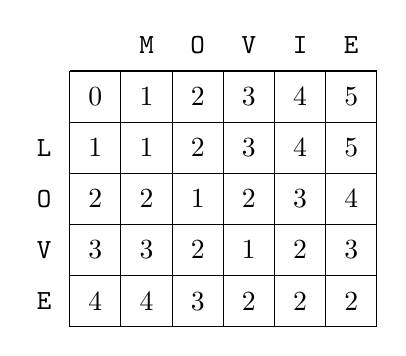
\begin{tikzpicture}[scale=.65]
  \begin{scope}
    %\fill [color=lightgray] (5, -3) rectangle (6, -4);
    \draw (1, -1) grid (7, -6);
    
    \node at (0.5,-2.5) {\texttt{L}};
    \node at (0.5,-3.5) {\texttt{O}};
    \node at (0.5,-4.5) {\texttt{V}};
    \node at (0.5,-5.5) {\texttt{E}};

    \node at (2.5,-0.5) {\texttt{M}};
    \node at (3.5,-0.5) {\texttt{O}};
    \node at (4.5,-0.5) {\texttt{V}};
    \node at (5.5,-0.5) {\texttt{I}};
    \node at (6.5,-0.5) {\texttt{E}};

    \node at (1.5,-1.5) {$0$};
    \node at (1.5,-2.5) {$1$};
    \node at (1.5,-3.5) {$2$};
    \node at (1.5,-4.5) {$3$};
    \node at (1.5,-5.5) {$4$};
    \node at (2.5,-1.5) {$1$};
    \node at (2.5,-2.5) {$1$};
    \node at (2.5,-3.5) {$2$};
    \node at (2.5,-4.5) {$3$};
    \node at (2.5,-5.5) {$4$};
    \node at (3.5,-1.5) {$2$};
    \node at (3.5,-2.5) {$2$};
    \node at (3.5,-3.5) {$1$};
    \node at (3.5,-4.5) {$2$};
    \node at (3.5,-5.5) {$3$};
    \node at (4.5,-1.5) {$3$};
    \node at (4.5,-2.5) {$3$};
    \node at (4.5,-3.5) {$2$};
    \node at (4.5,-4.5) {$1$};
    \node at (4.5,-5.5) {$2$};
    \node at (5.5,-1.5) {$4$};
    \node at (5.5,-2.5) {$4$};
    \node at (5.5,-3.5) {$3$};
    \node at (5.5,-4.5) {$2$};
    \node at (5.5,-5.5) {$2$};
    \node at (6.5,-1.5) {$5$};
    \node at (6.5,-2.5) {$5$};
    \node at (6.5,-3.5) {$4$};
    \node at (6.5,-4.5) {$3$};
    \node at (6.5,-5.5) {$2$};
  \end{scope}
\end{tikzpicture}
\end{center}

Төменгі оң жақтағы бұрышта \texttt{LOVE}
мен \texttt{MOVIE} арасындағы түзету 
арақашықтығының 2 екенін көрсетеді. Сондай-ақ кестеде 
түзету операцияларының ең қысқа 
тізбегін құру жолы берілген.
Түзету жолы:

\begin{center}
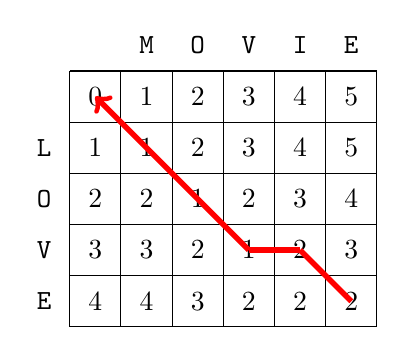
\begin{tikzpicture}[scale=.65]
  \begin{scope}
    \draw (1, -1) grid (7, -6);
    
    \node at (0.5,-2.5) {\texttt{L}};
    \node at (0.5,-3.5) {\texttt{O}};
    \node at (0.5,-4.5) {\texttt{V}};
    \node at (0.5,-5.5) {\texttt{E}};

    \node at (2.5,-0.5) {\texttt{M}};
    \node at (3.5,-0.5) {\texttt{O}};
    \node at (4.5,-0.5) {\texttt{V}};
    \node at (5.5,-0.5) {\texttt{I}};
    \node at (6.5,-0.5) {\texttt{E}};

    \node at (1.5,-1.5) {$0$};
    \node at (1.5,-2.5) {$1$};
    \node at (1.5,-3.5) {$2$};
    \node at (1.5,-4.5) {$3$};
    \node at (1.5,-5.5) {$4$};
    \node at (2.5,-1.5) {$1$};
    \node at (2.5,-2.5) {$1$};
    \node at (2.5,-3.5) {$2$};
    \node at (2.5,-4.5) {$3$};
    \node at (2.5,-5.5) {$4$};
    \node at (3.5,-1.5) {$2$};
    \node at (3.5,-2.5) {$2$};
    \node at (3.5,-3.5) {$1$};
    \node at (3.5,-4.5) {$2$};
    \node at (3.5,-5.5) {$3$};
    \node at (4.5,-1.5) {$3$};
    \node at (4.5,-2.5) {$3$};
    \node at (4.5,-3.5) {$2$};
    \node at (4.5,-4.5) {$1$};
    \node at (4.5,-5.5) {$2$};
    \node at (5.5,-1.5) {$4$};
    \node at (5.5,-2.5) {$4$};
    \node at (5.5,-3.5) {$3$};
    \node at (5.5,-4.5) {$2$};
    \node at (5.5,-5.5) {$2$};
    \node at (6.5,-1.5) {$5$};
    \node at (6.5,-2.5) {$5$};
    \node at (6.5,-3.5) {$4$};
    \node at (6.5,-4.5) {$3$};
    \node at (6.5,-5.5) {$2$};

    \path[draw=red,thick,-,line width=2pt] (6.5,-5.5) -- (5.5,-4.5);
    \path[draw=red,thick,-,line width=2pt] (5.5,-4.5) -- (4.5,-4.5);
    \path[draw=red,thick,->,line width=2pt] (4.5,-4.5) -- (1.5,-1.5);
  \end{scope}
\end{tikzpicture}
\end{center}

\texttt{LOVE} пен \texttt{MOVIE}-дің соңғы таңбалары бірдей,
сондықтан олардың түзету арақашықтығы 
\texttt{LOV} және \texttt{MOVI} арасындағы
түзету арақашықтығымен бірдей болады.
Бір түзету операциясымен \texttt{MOVI}-ден
\texttt{I} таңбасын өшірсек жеткілікті. 
Демек түзету арақашықтығы \texttt{LOV} және \texttt{MOV} арасындағы 
түзету арақашықтығынан 1-ге үлкен. Ары қарай да дәл осылай жалғаса береді. 

\section{Тақташа төсеу жолдарын санау}

Кейде динамикалық бағдарламалаудың шешімдегі күйлері 
жай тұрақты сандардан күрделірек болады. Мысал үшін  келесі
есепті қарастырайық:
$n \times m$ торда өлшемі $1 \times 2$ мен $2 \times 1$ 
тақташаларын төсеу жолдарын табуымыз қажет.
$4 \times 7$ торы үшін төсеудің жарамды жолын
 қарастырайық :
\begin{center}
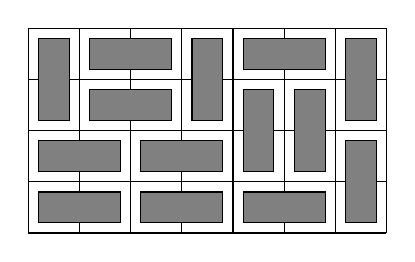
\begin{tikzpicture}[scale=.65]
    \draw (0,0) grid (7,4);
    \draw[fill=gray] (0+0.2,0+0.2) rectangle (2-0.2,1-0.2);
    \draw[fill=gray] (2+0.2,0+0.2) rectangle (4-0.2,1-0.2);
    \draw[fill=gray] (4+0.2,0+0.2) rectangle (6-0.2,1-0.2);
    \draw[fill=gray] (0+0.2,1+0.2) rectangle (2-0.2,2-0.2);
    \draw[fill=gray] (2+0.2,1+0.2) rectangle (4-0.2,2-0.2);
    \draw[fill=gray] (1+0.2,2+0.2) rectangle (3-0.2,3-0.2);
    \draw[fill=gray] (1+0.2,3+0.2) rectangle (3-0.2,4-0.2);
    \draw[fill=gray] (4+0.2,3+0.2) rectangle (6-0.2,4-0.2);

    \draw[fill=gray] (0+0.2,2+0.2) rectangle (1-0.2,4-0.2);
    \draw[fill=gray] (3+0.2,2+0.2) rectangle (4-0.2,4-0.2);
    \draw[fill=gray] (6+0.2,2+0.2) rectangle (7-0.2,4-0.2);
    \draw[fill=gray] (4+0.2,1+0.2) rectangle (5-0.2,3-0.2);
    \draw[fill=gray] (5+0.2,1+0.2) rectangle (6-0.2,3-0.2);
    \draw[fill=gray] (6+0.2,0+0.2) rectangle (7-0.2,2-0.2);

\end{tikzpicture}
\end{center}
Жалпы жолдар саны -- 781.

Есепті тордағы жолдардан кезек-кезек өтетін 
динамикалық бағдарламалау арқылы шығаруға болады. 
Жауаптағы әр жол $\{\sqcap, \sqcup, \sqsubset, \sqsupset \}$
жиынындағы $m$ таңбадан тұратын жол ретінде көрсетіле алады. 
Жоғарыдағы жауап төмендегі төрт жолға
сәйкес келеді:
\begin{itemize}
\item
$\sqcap \sqsubset \sqsupset \sqcap \sqsubset \sqsupset \sqcap$
\item
$\sqcup \sqsubset \sqsupset \sqcup \sqcap \sqcap \sqcup$
\item
$\sqsubset \sqsupset \sqsubset \sqsupset \sqcup \sqcup \sqcap$ 
\item
$\sqsubset \sqsupset \sqsubset \sqsupset \sqsubset \sqsupset \sqcup$
\end{itemize}


$\texttt{count}(k,x)$ деп
$k$-жол $x$-ке сәйкес болатын
тордағы $1 \ldots k$ жолдары үшін
төсеу санын анықтайық.
Бұл жерде динамикалық бағдарламалауды қолдануға 
болады. Себебі жолдың күйі 
тек алдыңғы жолдың күйімен шектеледі

Егер $1$-жолда $\sqcup$ таңбасы болмаса, 
$n$-жолда $\sqcap$ таңбасы болмаса 
және қатар жолдар \emph{үйлесімді} болса, 
жауап жарамды болады. 
Мысалы, $\sqcup \sqsubset \sqsupset \sqcup \sqcap \sqcap \sqcup$ 
$\sqsubset \sqsupset \sqsubset \sqsupset \sqcup \sqcup \sqcap$ жолдары үйлесімді, ал
$\sqcap \sqsubset \sqsupset \sqcap \sqsubset \sqsupset \sqcap$,
$\sqsubset \sqsupset \sqsubset \sqsupset \sqsubset \sqsupset \sqcup$ жолдары үйлесімді емес.

Жол $m$ таңбадан тұрғандықтан және әрбір таңбаға 4
нұсқа қоюға болатындықтан, жол түрлері санының ең көбі $4^m$ болады.
Демек шешімнің уақытша күрделілігі $O(n 4^{2m})$. Себебі
әр жолдың $O(4^m)$ күйі бар және алдыңғы жолдың да 
$O(4^m)$ күйі бар. Іс барысында 
кіші жағы $m$ болатындай етіп торды айналдырған дұрыс. 
Өйткені $4^{2m}$ факторы басым болады. 

Егер жолдардың көрінісін ықшамдасақ,
есепті тиімдірек шығаруға болады. 
Бұл жағдайда алдыңғы жолдың қай бағаналарында 
тік тақтайшаның жоғарғы шаршысы бар 
екенін білу жеткілікті.
Яғни жолды тек $\sqcap$ және $\Box$ таңбалары 
арқылы көрсетсек болады, мұнда $\Box$ -- 
$\sqcup$, $\sqsubset$ және $\sqsupset$ таңбаларының комбинациясы бар. % TODO
Осы көріністі қолдана отырып, әр жолдың
$2^m$ түрі болуына сәйкес уақытша күрделілігі
$O(n 2^{2m})$ тең болады. 


Сөз соңында бұл есепті төмендегі таңғажайып формула арқылы шығаруға да болатынын айта кеткіміз келеді:
\footnote{Бұл формуланы 1961 жылы өз бетінше жұмыс істеген екі зерттеу тобы ашты.
\cite{kas61,tem61}}:
\[ \prod_{a=1}^{\lceil n/2 \rceil} \prod_{b=1}^{\lceil m/2 \rceil} 4 \cdot (\cos^2 \frac{\pi a}{n + 1} + \cos^2 \frac{\pi b}{m+1})\]
Аталмыш формула аса тиімді. Ол төсеу жолдарын $O(nm)$
уақытта табады. Бірақ жауап нақты сандардың көбейтіндісінен
тұратындықтан, олардың аралық нәтижелерін дәлдікпен сақтау қиынға соғады.



